There are several types of Malware that can be used to compromise a network or
a computer.The propagation of a malware can also happen through social
engineering, being phishing one of the most common examples \citep{greenbergSandwormNewEra2019}.
This lab objective is to discover and research different types of specific
malwares.

\section{Zeus Gameover}
\label{s:Zeus-Gameover}
One of the most famous malware is Zeus Gameover. Zeus is a trojan that spreads
itself through emails with malicious attachments \citep{wikipediaGameoverZeuS2021}.
This malware will then generate zombies that sit in an IRC server managed by a
server administrator. This process is a continue and infinite loop and makes the
battle against the botnets really hard \citep{firatInevitableBattleBotnets2020}.
Zeus uses anAdobe Reader BMP/RLE heap corruption vulnerability CVE-2013-2729 that
causes a buffer overflow to cause a DoS that makes the daemon crash and execute
malicious code \citep{ismailEffectsFeatureSelection2021}.
In the case of Zeus, most of the time, a PDF file is used to initialise
everything and start the new botnet. It will use the vulnerabilities of the
reader to declare previously where the shellcode is not even hidden, and that
can be easily decrypted \citep{eternalSpammedCVE20132729PDF2013}. These
discoveries are made using a python tool named peepdf that analyse a pdf file.
The principal scope of the botnet is to steal banking informations where the
victims are deprived of their money when the amount is worth to be taken \citep{
knowbe4GameoverZeusGOZ2020}.

\begin{figure}[ht]
  \centering
  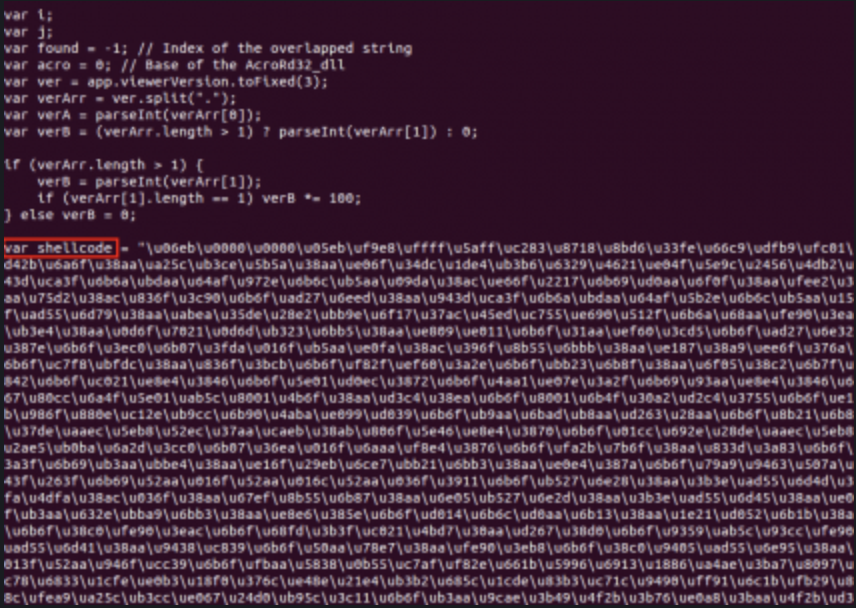
\includegraphics[width=0.5\textwidth]{figures/shellcode-zeus}
  \caption{Shellcode Zeus Gameover}
  \label{f:shellcode-zeus}
\end{figure}
